\documentclass[aip,jcp,reprint,amsmath,amssymb,amsfonts,showkeys]{standalone}

\usepackage{graphicx,bm,microtype,hyperref,algpseudocode,subfigure,algorithm,algorithmicx,multirow,footnote,xcolor,physics,ulem}
\usepackage[version=4]{mhchem}

\newcommand{\cS}{\Hat{S}}
\newcommand{\cT}{\Hat{\Theta}}
\newcommand{\cK}{\Hat{K}}

\usepackage{tikz}
\usetikzlibrary{arrows,positioning,shapes.geometric}
\usetikzlibrary{decorations.pathmorphing}

% Set the overall layout of the tree
\tikzstyle{level 1}=[level distance=5cm, sibling distance=4cm]
\tikzstyle{level 2}=[level distance=5cm, sibling distance=2cm]
\tikzstyle{level 3}=[level distance=5cm, sibling distance=2cm]
\tikzstyle{end} = [circle, minimum width=4pt,fill, inner sep=0pt]

\usepackage{tikz}
\usetikzlibrary{arrows,positioning,shapes.geometric}
\usetikzlibrary{decorations.pathmorphing}

\tikzset{snake it/.style={
decoration={snake, 
    amplitude = .4mm,
    segment length = 4mm},decorate}
}
  \newcommand\redsout{\bgroup\markoverwith
      {\textcolor{red}{\rule[0.5ex]{2pt}{0.4pt}}}\ULon}  
\begin{document}

%%% FIGURE 3 %%%
\resizebox{\linewidth}{!}{
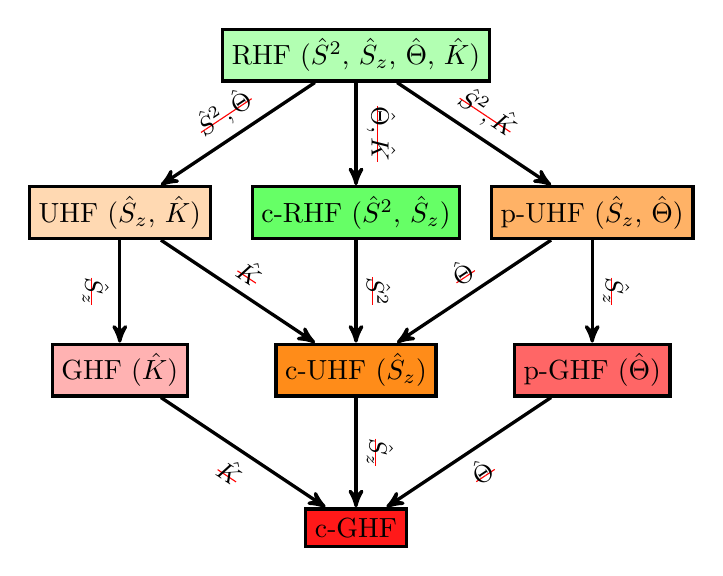
\begin{tikzpicture}
	\begin{scope}[
		very thick,
		node distance=2cm and 3cm,on grid,>=stealth',
		box_RHF/.style={rectangle,draw,fill=green!30},
		box_UHF/.style={rectangle,draw,fill=orange!30},
		box_cRHF/.style={rectangle,draw,fill=green!60},
		box_pUHF/.style={rectangle,draw,fill=orange!60},
		box_GHF/.style={rectangle,draw,fill=red!30},
		box_cUHF/.style={rectangle,draw,fill=orange!90},
		box_pGHF/.style={rectangle,draw,fill=red!60},
		box_cGHF/.style={rectangle,draw,fill=red!90}
		],
		\node [box_RHF,  align=center]		(RHF)									{RHF ($\cS^2$, $\cS_z$, $\cT$, $\cK$)};
		\node [box_cRHF, align=center]		(cRHF)		[below=of  RHF]				{c-RHF ($\cS^2$, $\cS_z$)};
		\node [box_UHF,  align=center]		(UHF)		[left=of  cRHF]				{UHF ($\cS_z$, $\cK$)};
		\node [box_pUHF, align=center]		(pUHF)		[right=of cRHF]				{p-UHF ($\cS_z$, $\cT$)};
		\node [box_cUHF, align=center]		(cUHF)		[below=of cRHF]				{c-UHF ($\cS_z$)};
		\node [box_GHF,  align=center]		(GHF)		[left=of  cUHF]				{GHF ($\cK$)};
		\node [box_pGHF, align=center]		(pGHF)		[right=of cUHF]				{p-GHF ($\cT$)};
		\node [box_cGHF,  align=center]		(cGHF)		[below=of cUHF]				{c-GHF};
		\path 
		(RHF)		edge[->]			node[above,sloped]{\small \redsout{$\cT,\cK$}}		(cRHF)
		(RHF)		edge[->]			node[above,sloped]{\small \redsout{$\cS^2,\cT$}}		(UHF)
		(RHF)		edge[->]			node[above,sloped]{\small \redsout{$\cS^2,\cK$}}		(pUHF)
		(cRHF)		edge[->]			node[above,sloped]{\small \redsout{$\cS^2$}}			(cUHF)
		(UHF)		edge[->]			node[below,sloped]{\small \redsout{$\cS_z$}}			(GHF)
		(UHF)		edge[->]			node[above,sloped]{\small \redsout{$\cK$}}			(cUHF)
		(pUHF)		edge[->]			node[above,sloped]{\small \redsout{$\cS_z$}}			(pGHF)
		(pUHF)		edge[->]			node[above,sloped]{\small \redsout{$\cT$}}			(cUHF)
		(cUHF)		edge[->]			node[above,sloped]{\small \redsout{$\cS_z$}}			(cGHF)
		(GHF)		edge[->]			node[below,sloped]{\small \redsout{$\cK$}}			(cGHF)
		(pGHF)		edge[->]			node[below,sloped]{\small \redsout{$\cT$}}			(cGHF)
		;
	\end{scope}
\end{tikzpicture}
}
%%%


\end{document}
